\documentclass[12pt,a4paper]{report}
%\fontencoding{T1}

\usepackage[utf8x]{inputenc}
\usepackage[T1]{fontenc}
\usepackage[danish]{babel}
\usepackage[hidelinks]{hyperref}
%\usepackage{lingmacros}
%\usepackage{tree-dvips}
\usepackage{url}
\usepackage{array}
\usepackage{graphicx}
\usepackage{float}
\usepackage{lastpage}
\usepackage{color}
\usepackage[x11names,rgb,usenames,dvipsnames,svgnames,table]{xcolor}
\usepackage{colortbl}
\usepackage{algorithm2e}
\usepackage{geometry}
\usepackage{titlesec, blindtext, color}
\definecolor{gray75}{gray}{0.75}
\definecolor{gray90}{gray}{0.90}
\definecolor{ForestGreen}{RGB}{15,116,61}
\definecolor{gray25}{gray}{0.25}
\newcommand{\hsp}{\hspace{20pt}}

\usepackage{tikz}
\usetikzlibrary{snakes,arrows,shapes}
\usepackage{amsmath}

\usepackage{xcolor} 
\usepackage{fix-cm} 
\usepackage{pgfplots}

%Titelblad fix
%\usepackage[ansinew]{inputenc}
\usepackage{a4}

\titleformat{\chapter}[hang]{\Huge\bfseries}{\thechapter\hsp\textcolor{gray75}{|}\hsp}{0pt}{\Huge\bfseries}

\begin{document}
\setcounter{page}{2}

\begin{titlepage}
\newcommand{\HRule}[1]{\hfill \rule{0.2\linewidth}{#1}} 

\definecolor{grey}{rgb}{0.9,0.9,0.9} 
\newgeometry{top=2in,bottom=1in,right=0cm,left=0cm}
\thispagestyle{empty} 

\noindent \colorbox{grey}{
	 \parbox[t]{1.0\linewidth}{
		\centering \fontsize{50pt}{80pt}\selectfont
		\vspace*{0.7cm}
		P1-Procesanalyse \\[3pt]
		\vspace*{0.7cm}
	}
}

\vfill
\flushright
\flushright \rule[10pt]{0.1pt}{160pt}  \begin{minipage}[b]{0.45\linewidth}
{
\Large
\textbf{Gruppe B228:} \\[4pt]
Anders Trier Olesen\\[.2cm]
Katrine Sofie Tjell\\[.2cm]
Jannek Alexander Westerhof Bossen\\[.2cm]
Kevin Brämer\\[.2cm]
Frederik Meyer Bønneland\\[.2cm]
Ólavur Debes Joensen\\[.2cm]
}
\end{minipage}

\clearpage 

%\title{P1-Rapport}
%\author{B228}
%\date{\today}
%\pagebreak
%\maketitle
%% Fjerner sidetal på forsiden
\thispagestyle{empty}
\end{titlepage}


\tableofcontents
% Fjerner sidetal på indholdsfortegnelse
\thispagestyle{empty}

\renewcommand{\chaptername}{Kapitel}

% TEKST SÆTTES UNDER HER
\chapter{Indledning}
\setcounter{page}{3}
	Formålet med denne analyse er at dokumentere P2 projektforløbet for gruppe A325. Derudover er meningen med analysen, at gruppen reflekterer over samarbejdet og arbejdsgangen gennem projektforløbet.
\\
Gruppen består af 6 personer som var sammen i P1-projektet samt én ny person. I P1-projektforløbet fungerede gruppen rigtig godt og derfor blev det besluttet at fortsætte sammen i P2 sammen med blot én ny person. Derved kendte størstedelen af gruppen hinanden og det gjorde at det var let at komme i gang med projektet, da  der ikke skulle bruges tid på at lære hinanden at kende. At en ny person kom ind i gruppen forvoldte ingen problemer, men gjorde tværtimod at der kom nogle nye ideér og meninger på banen. Forventning til projektforløbet var fra starten, at det skulle forløbe nogenlunde som det havde gjort i P1, at ambitionsniveauet skulle være højt og at projektet skulle ende med at ligge over middel. 
\\
Forventningen til udbyttet af projektet, var at gruppen ville lære mere om problemanalyse og det at skrive rapport. Derudover var alle opsat på at gøre brug af de erfaringer vi gjorde i P1 projektet og på den måde lave et bedre projekt. 
 %Indhold af Indledning.tex bliver sat ind her.
	

\chapter{Projektplanlægning og projektstyring}
\label{projektplan}
 
    \section{Beskrivelse}
Som følge af erfaring fra P1-projektet, skulle vi i P2 følge en tidplan for projektperioden. Derved blev der i starten af projektet, ved hjælp af programmet \textit{Ganter}, udviklet en tidsplan for projektet, hvori de forskellige deadlines for projektet blev lagt ind i. Men ligesom på P1-projektet lykkedes det desværre heller ikke denne gang at hverken følge tidsplanen eller holde denne opdateret. I stedet delte vi blot opgaver ud fra dag til dag og aftalt deadlines samtidigt. Når vi så mødtes for at arbejde i grupperummet opgjorde vi status af projektet og aftalte hvornår vi skulle mødes næste dag. 

Som følge af erfaring fra P1 har vi til fildeling mellem gruppensmedlemmer brugt GitHub og det virkede atter rigtig godt. Samtidigt har vi brugt \LaTeX{} som formateringssporg til at skrive rapport i.   

Ligesom i P1 havde vi helle ikke i dette projektforløb en projektleder. Grunden er at alle er enige om at i P1 fungerede det godt at der ikke er én person der har styringen, med at alle istedet har ansvaret for at holde arbejdet i gang. Ingen andre grupperoller blev delt ud.  

Lidt over en måned inde i projektforløbet, blev der afholdt statusseminar. Her blev problemanalyse for projeket og vores ideér til det videre arbejde fremlagt for en opponentgruppe, samt vejledere. Derefter fik vi kommentere og nye overvejelser med hjem. Derudover så vi fremlæggelse fra en anden gruppe og kunne derved hente lidt inspiration fra dem, til brug i vores eget projekt. Efter statusseminaret rettede vi selvfølgelig det, som vi havde fundet ud af kunne blive bedre, og derefter gik vi lidt i stå. GitHub.com danner en graf over hvor meget aktivitet, der har været i projektet i forhold til tiden, se bilag \ref{bilag2}. Denne graf ligner meget den tilsvarende graf fra P1, på trods af at vi efter P1 ønskede at ændre denne arbejdsaktivitet. Grafen på bilag \ref{bilag2} viser, at vi kom lidt langsomt fra start, men at fik lavet rigtig meget inden statusseminaret. Efter seminaret er aktiviteten kraftigt dalende hen mod midten af april hvor aktiviten nærmest står stille i den uge hvor vi skulle lave eksamensprojekt i OOP. Hen imod aflevering af projektet stiger aktiviteten kraftigt. 

\section{Analyse}

\emph{Gode erfaringer:}
\begin {itemize}
\item  GitHub er fortsat glimrende til fildeling.

\item	Godt at ansvar for styring af gruppen ikke placeres på én eventuel projektleder. 

\item	Statusseminaret var godt. Gruppen øvede sig i at fremlægge projekt og der kom nye ideér på banen.
\end{itemize}\emph{Dårlige erfaringer:}
\begin{itemize}
\item	Også i dette projekt så vi en skiftende abrjedsindsats, som først kom i top hen mod en deadline (statusseminar eller endelig aflevering). Det havde været bedre med en konstant arbejdsindsats. 

\item	Den manglende styr på tidplanen, gjorde at vi indimellem mistede overblikket over projeket. 

\item	Ikke at dele nogle roller ud i gruppen. En rolle kunne være at holde styr på tidplanen.
\end{itemize}

\section{Forbedringer til P3}

I næste projekt kunne det være en god idé at forsøge med udelling af roller mellem gruppens medlemmer. Eksempelvis kunne man have en sekretær, som kunne sikre at der bliver styr på tidplanen, samt holde kontakt til vejleder osv. Man kunne derudover vælge en person til at være ordstyrer og derved sikre at diskussioner i gruppen, foregår på en ordentlig måde. Man kunne eventuelt skiftes til at påtage sig de forskellige roller. 

Ved at vælge én person til at holde styr på tidsplanen kunne man måske sikre at dette rent faktisk bliver gjort. Det kunne være godt at undgår at miste overblikket, som det ind imellem er sket i denne projektperiode. Derved kunne man også få flere deadlines på tidplanen, således at arbejdsindsatsen ikke bliver så ”bølget”.




\chapter{Samarbejde i gruppen}
 
    \section{Beskrivelse}
I P1 udarbejdede vi i gruppen en gruppekontrakt. Denne fik vi dog ikke særlig meget glæde af, da ingen egentlig følte, at der var brug for den. Derfor blev der til P2 ikke lavet nogen kontrakt og i stedet aftalte vi mundtligt at der var ”mødepligt” til både forelæsninger, vejledermøder og gruppemøder. Hvilket vil sige, at hvis man ikke kunne komme, skulle der meldes afbud.

Til projektarbejdet i grupperummet havde vi ingen faste mødetidspunkter, men i stedet aftalte vi fra dag, til dag om der skulle mødes næste dag og i så fald hvornår. Hvis vi ikke skulle mødes dagen efter, aftalte vi så hvad hver især skulle lave derhjemme.
Facebook er blevet brugt i stor stil til indbyrdes kommunikation med hinanden, når vi sad hjemme og ikke var samlet i grupperummet. Her har vi eksempelvis delt forskellige hjemmesider mellem hinanden. 
Ellers har vi i grupperummet gjort rigtig meget brug af tavlerne, som har været et godt værktøj til at skabe overblik. Som eksempel har vi skrevet spørgsmål til vejleder op på tavlen, for ikke at glemme dem, og ligeledes ofte lavet en to-do liste over dagen. 

Engang imellem har vi i gruppen også husket at lægge arbejdet til side, og lave sociale ting sammen. Det har vi gjort for ikke at gå død i arbejdet og samtidigt styrke sammenholdet og samarbejdet i gruppen. Vi har eksempelvis haft ”spille-aften”, spist aftensmad sammen, gået i fredagsbar og i byen sammen. Derved sørger vi for at alt ikke bare drukner i fagligt arbejde, men at vi også kan have det sjovt sammen.

Kommunikationen i gruppen har fungeret godt, ingen er blevet uvenner eller overhørt. Alle er af den mening at alle i gruppen siger deres mening og at alle hører efter når nogen taler. Derved gives der plads til alle i gruppen, og  samarbejdet har fungeret optimalt gennem hele projektforløbet.

\section{Analyse}

\emph{Gode erfaringer:}
\begin{itemize}

\item	Det er fint ikke at have en gruppekontrakt, da gruppen kendte hinanden i forvejen.

\item	Det fungerer godt at man ikke nødvendigvis skal møde hver dag, hvis der alligevel ikke er forelæsning. Nogen i gruppen synes bedre om at arbejde hjemme.  

\item	Godt at alles meninger bliver respekteret og hørt.

\item	Sociale arrangementer udenfor arbejdstiden er gode og vigtige at holde fast i.

\item	 Brugen af tavlerne i grupperummet skal vi fortsætte med, da det gør at alle er med på hvad der foregår. 
\end{itemize}\emph{Dårlige erfaringer:}
\begin{itemize}

\item	 Nogle gange er folk meget dårlige til at give svar på forespørgsler på Facebook. Dette var frustrerende for den, som stillede spørgsmålet.

\item	Mødetiderne blev ikke altid overholdt, hvilket gav frustration for den del af gruppen der var mødt til tiden.
\end{itemize}

\section{Forbedringer til P3}
Det er en god idé med gruppekontrakt, hvor man kunne aftale faste mødetider, så dette ikke skal aftales over Facebook. Derudover bør der være en konsekvens hvis man ikke kommer til tiden.



\chapter{Samarbejde med vejlederen}
 
    \section{Beskrivelse}
Samarbejdet med vores vejleder har været godt. Vi valgte sammen med vejlederen, at der ikke var behov en decideret kontrakt, men at vi bare ville tage det som det kom. Vi aftalte at gruppen skulle skrive dagsorden inden hvert møde og ligeledes skrive referat under hvert møde. Derudover var det primært vejleder der bestemte hvornår vi skulle holde møder, da han havde lang transporttid og 3 andre grupper at koordinere med. Inden vi havde første møde med vejleder gjorde vi os nogle få overvejelser om hvordan vi ville bruge ham:
\begin{itemize}
\item	Efter behov ville vi gerne sende henholdsvis rapport og kode, til gennemlæsning af vejleder, med håb om efterfølgende feedback.

\item	Vi vil gerne have regelmæssige møder, med henblik på hele tiden at holde os på rette spor med hjælp fra vejleder.

\item Til sidst ville vi gerne have mulighed for løbende at sende spørgsmål over mail, når de skulle melde sig.
\end{itemize}
Vejleder var enig i måden at bruge ham på og vi blev enige om at samarbejdet skulle fungere sådan. Det har kørt sådan at vejleder sendte en mail til os om, hvornår vi skulle holde møde. Mindst en dag inden mødet sendte vi en mail til vejleder, med den nyeste rapport og eventuelle spørgsmål. Til mødet talte vi så om hvad status på projektet var. 

En i gruppen blev valgt til referent og var således referent til hvert møde, så vi altid fik skrevet referat. Vi mener selv, at vi i dette projekt har fået rettet op på de dårlige erfaringer vi gjorde i P1.


[[HVILKE DÅRLIGE ERFARINGER???]]


En dårlig erfaring var eksempelvis at vi fik holdt alt for få vejledermøder, hvilket gjorde at vi nogle gange arbejdede ud af et forkert spor, eller simpelthen fik lavet for lidt. 

\section{Analyse}

\emph{Gode erfaringer:}
\begin{itemize}

\item Godt med ugentlige vejledermøder. På den måde fik vi hele tiden holdt status over projektet og kom hele tiden videre.

\item Godt, at den samme person var referent hver gang, hvilket gjorde at referatet altid var opbygget på samme måde og gav et fint overblik.
\end{itemize}
\emph{Dårlige erfaringer:}
\begin{itemize}
\item	Der var som oftest sat en hel time af til vejledermøderne. Ofte var vi færdige med det projekt-relevante stof indenfor en halv time, hvorefter resten af mødet gik med snak om alt muligt andet. Nogle i gruppen synes det var hyggeligt med den "ligegyldige" snak, mens andre i gruppen synes det var tidsspilde.

\end{itemize}

\section{Forbedringer til P3}

I næste projekt skal vi sørge for, at tale med vejleder om, hvor lange vi mener møderne bør være, således at gruppen ikke føler at tiden spildes. Der skal holdes fast i at få holde ugentlige vejldermøder, da dette fungerede rigtig godt. 



\chapter{Læreprocessen}
 
    \section{Beskrivelse}
Ved siden af projektarbejdet, har alle i gruppen deltaget i 3 kurser; Diskret Matematik (DMAT), Computer Arkitektur (CART) og Objekt Orienteret Programmering (OOP). Med hensyn til projektet har vi klart fået mest ud af OOP. Dette kursus handlede naturligvis om programmering og sproget der blev brugt var C\#. C\# var netop det sprog som programmet der skulle udvikles i forbindelse med P2 skulle skrives i. Derved lærte vi det, som var nødvendigt for at vi kunne udleve kravene til P2. DMAT og CART er kurser, som er relevante for vores udennelse generelt og i senere projekter kommer vi til at kunne gøre godt brug af dem. Men til dette projekt har vi ikke rigtigt kunnet bruge hverken DMAT eller CART.
I forbindelse med alle kurserne sad gruppen sammen og løste kursernes opgaver i fællesskab. Det er dog lige med undtagelse af CART, hvor nogen i gruppen havde lidt svært ved at fastholde koncentrationen og interessen.
Med hensyn til selve projektarbejdet, delte vi arbejdet ud mellem gruppens medlemmer, på en såden måde at alle lavede lidt af det hele. I P1 delte gruppen sig på et tidspunkt i to således at den ene del arbejdede videre på rapporten og den anden del arbejdede på programmet. Dette resulterede i at det kun var den ene halvdel af gruppen der var godt inde i programmet. Det har vi forsøgt at ændre i P2.
Derudover tog vi en god erfaring med fra P1, hvilket er, at når et afsnit til rapporten er blevet færdiggjort, skal mindst to andre læse det igennem. På den måde får man rettet afsnittene løbende og alle lærer om hele projektet og ikke bare den del man selv har skrevet. 

\section{Analyse}

\emph{Gode erfaringer:}
\begin{itemize}
\item Det er godt at gruppen hjælper hinanden med kursus-opgaver. Det giver godt sammenhold og sammarbejde i gruppen. 

\item Det er godt at alle arbejde på alle sider af projektet, så alle er sat godt ind i det hele.

\item	Fortsat virker det godt, at mindst 2 personer læser og giver kommentarer til nye afsnit, inden disse bliver tilføjet rapporten.
\end{itemize}\emph{Dårlige erfaringer:}
\begin{itemize}
\item	Gruppen burde måske have forsøgt at få alle med i CART, så der ikke var nogen der kom bagefter.

\end{itemize}	 

\section{Forbedringer til P3}
Alle i gruppen skal selv tage et ansvar for at deltage aktivt i kurserne, så dette ikke kommer til at påvirke gruppen negativt senere hen. Derudover skal vi fortsat have fokus på at alle løbende forstår hele projektet og alle derved lærer det samme. Dette skal sikre at gruppemedlemmerne ved alt om hele projektet og ikke mest om den del af projektet de selv har skrevet. 



\chapter{Konklussion}
 
    Når vi ser tilbage på projektforløbet er vi tilfredse. Vi har ikke stødt på problemer eller konflikter, som vi ikke har været i stand til at løse.Som nævnt i denne analyse er der ting vi vil gøre bedre i næste projekt, men også mange ting vi vil fortsætte med at gøre i P3. Eksempelvis har vi været gode til at tale med hinanden og sørge for at alle var inde over beslutningerne og på den måde opnå fælles enighed. Det vil vi helt klart fortsætte med i fremtidige projekter. 

\chapter*{Bilag}
\newgeometry{top=1in,bottom=1in,right=1in,left=1in}
\pagestyle{empty} % Fjerner sidetal fra bilag
\chapter*{Bilag 1: Danske Bank forside}
\setcounter{page}{1}
\thispagestyle{empty} % Fjerner sidetal fra bilag
\begin{figure}[H]
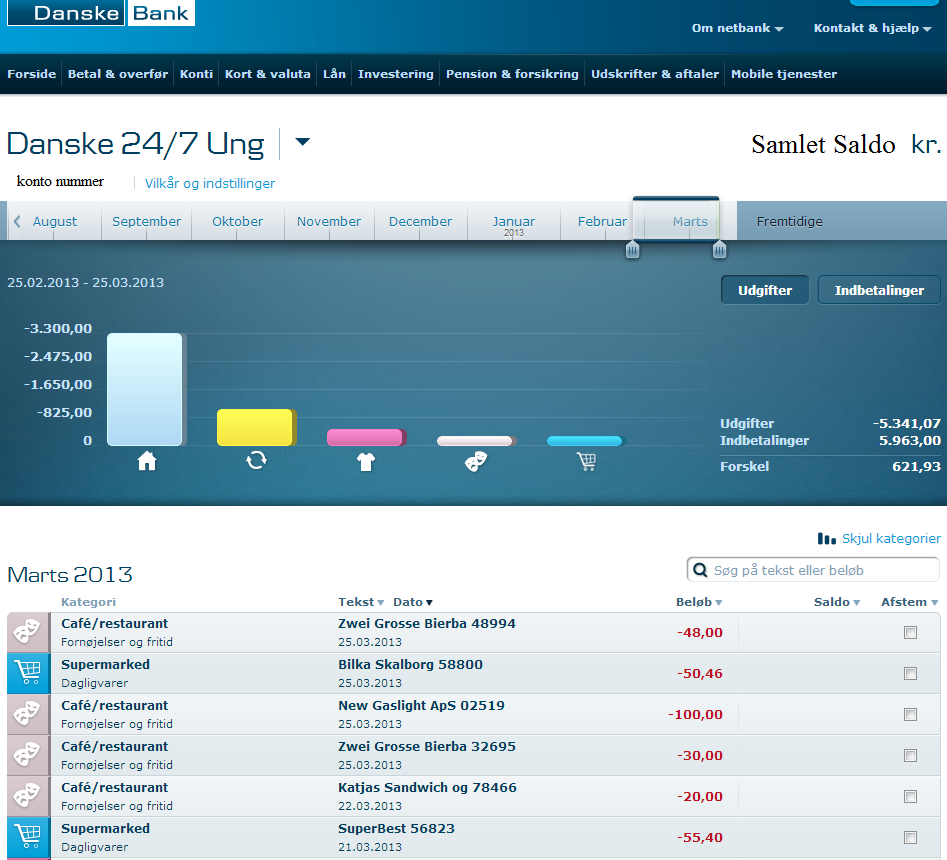
\includegraphics [width=\linewidth]{Billeder/bilagdb1.png}
\caption {Her ses et eksempel på den skærm man bliver mødt af når man logger ind på Danske Banks netbank}
\label {bilagdb1}
\end{figure}

\chapter*{Bilag 2: Databaseforbindelser}
\setcounter{page}{1}
\thispagestyle{empty} % Fjerner sidetal fra bilag
\begin{lstlisting}[caption={Statisk klasse, der forbinder til objekt databasen NDatabase},label={lst:db}]
public static class db
{
	//En string dbFileName med filnavnet på databasen laves
	private const string dbFileName = "database.db";
	
	//Herefter åbnes database forbindelsen
	private static NDatabase.Api.IOdb odb = OdbFactory.Open(dbFileName);

	public static void Store(Transfer transfer)
	{
		//Objektet bliver sendt til databasen
		odb.Store(transfer);
		
		//Databasen bliver tvunget til at opdatere
		odb.Commit();
	}
	
	public static Collection<Transfer> GetTransfersForChild(Child child)
	{
		//Lav en LINQ forespørgsel
		var transfers = from transfer in odb.QueryAndExecute<Transfer>()
						where transfer.Recipient != null && transfer.Recipient.FullName == child.FullName
						select transfer;

		//Lav en collection til at indeholde Transfers
		Collection<Transfer> Transfers = new Collection<Transfer>();

		//Flyt alle Transfers objekter fra transfers til Transfers (sikrer at forespørgslen bliver udført)
		foreach (var t in transfers)
			Transfers.Add(t);

		return Transfers;
	}
}
\end{lstlisting}
\vspace{1cm}
\begin{lstlisting}[caption={Statisk klasse, der forbinder til den relationelle database SQLite},label={lst:sqlite}]
public static class db
{
	//Navnet på filen databasen skal gemmes i
	private const string dbFileName = "test.sqlite";
	private static SQLiteConnection conn;

	//Metoder til at åbne og lukke forbindelsen til databasen
	public static void OpenDB()
	{
		conn = new SQLiteConnection("Data Source=" + dbFileName + ";Version=3;");
		conn.Open();
	}
	public static void CloseDB()
	{
		conn.Close();
	}

	public static void Store(Transfer transfer)
	{
		//Få fat i ID'et på Recipient 
		int ChildIDInDB = GetIDOfChild(transfer.Recipient);
		string ChildID = ((ChildIDInDB == 0) ? "null" : ChildIDInDB.ToString());

		//Selve SQL forespørgslen bliver lavet som en streng
		string query = "INSERT INTO Transfers (Title, Description, Amount, Recipient, Date, Type, Sender) VALUES ('" +
						transfer.Title + "', '" +
						transfer.Description + "', '" +
						transfer.Amount.ToString(CultureInfo.GetCultureInfo("en-GB")) + "', '" +
						ChildID + "', '" +
						SQLiteConvert.ToUnixEpoch((DateTime)transfer.TransferDate) + "', '" +
						//DateTimeToUnixTimeStamp((DateTime)transfer.TransferDate) + "', '" +
						(int)transfer.Type + "', '" +
						GetIDOfUser(transfer.Sender) + "')";
						
		//SQL kommandoen bliver udført
		SQLiteCommand command = new SQLiteCommand(query, conn);
		command.ExecuteNonQuery();
		NotifyTransferCreated(transfer);
	}

	//Metode der tager mod et objekt af typen Child, og returnerer Transfers
	public static Collection<Transfer> GetTransfersForChild(Child child)
	{
		//En SQL kommando opbygges
		string query = "SELECT * FROM Transfers WHERE " +
						"Recipient IN (SELECT ID FROM Childs WHERE " +
						"FirstName='" + child.FirstName + "'" +
						")";

		//Kommandoen udføres
		SQLiteCommand command = new SQLiteCommand(query, conn);
		SQLiteDataReader r = command.ExecuteReader();

		Collection<Transfer> TransferList = new Collection<Transfer>();

		//For hvert række returneret af databasen
		while (r.Read())
		{
			int ID = r.GetInt32(r.GetOrdinal("ID"));
			string Title = r.GetString(r.GetOrdinal("Title"));
			string Description = r.GetString(r.GetOrdinal("Description"));
			decimal Amount = r.GetDecimal(r.GetOrdinal("Amount"));
			Child Recipient = child;
			DateTime Date = SQLiteConvert.ToDateTime(((long)r["Date"]).ToString(), SQLiteDateFormats.UnixEpoch, DateTimeKind.Local);
			ActivityType Type = (ActivityType)(long)r["Type"];
			User Sender = ((long)r["Sender"] == 0) ? null : GetUser(r.GetInt32(r.GetOrdinal("Sender")));

		//Lav et nyt objekt af typen Transfer, og tilføj det til TransferList
		TransferList.Add(new Transfer(Title, Description, Amount, Recipient, Date, Type, Sender));
	}

	return TransferList;
}
\end{lstlisting}

\end{document}
 %\chapter{}
%	\section{SMS teknologi}
%	\input{Indhold/SMS_Teknologi}
